\section{Réactions chimiques oscillantes}

Nous étudions ici des réactions chimiques oscillantes, notamment la réaction de Belousov-Zhabotinsky, à travers un modèle simplifié à trois dimensions :

\begin{equation}
    \begin{aligned}
        \frac{dX}{dt} &= 10 + bZ - X - XY^2\ \text{, }
        \frac{dY}{dt} &= 200(X + XY^2 - Y) \ \text{, }
        \frac{dZ}{dt} &= 50(Y - Z) \
    \end{aligned}
\end{equation}

Avec des conditions initiales fixées à $[1; 0; 0]$, nous étudions l'évolution du système en fonction du paramètre $b$.

\subsection{Résolution numérique et premiers résultats}

Le système est résolu numériquement à l'aide de la méthode de Runge-Kutta d'ordre 4. La figure suivante montre l'évolution de $Y(t)$ pour différentes valeurs de $b$ :

\begin{figure}[H]
\centering
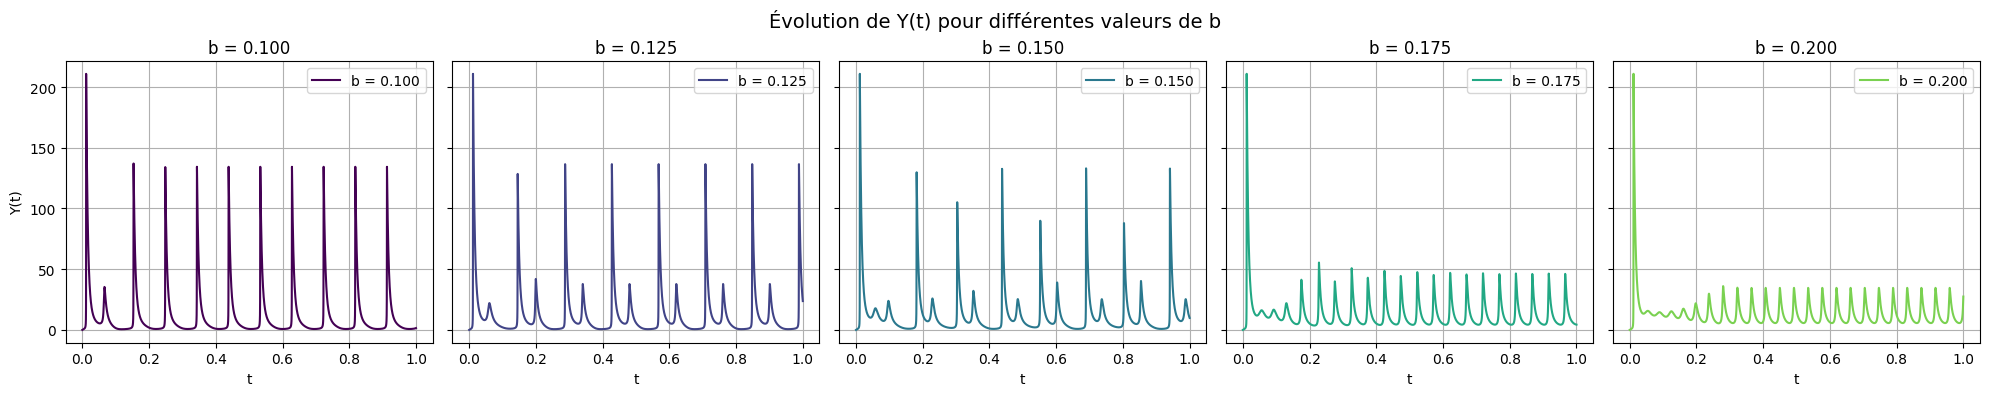
\includegraphics[width=\textwidth]{../code/resolution.png}
\caption{Comportement du système selon $b$}
\label{fig:oscillations}
\end{figure}

On observe que le système oscille, et que l'amplitude ainsi que la fréquence des pics de $Y(t)$ varient avec $b$ : plus $b$ augmente, plus les oscillations deviennent complexes.

\subsection{Analyse des périodes et bifurcations}

Une fonction \verb|periode_solution(b)| détecte les intervalles entre pics de $Y(t)$ à l'aide de \verb|find_peaks| (\texttt{scipy}). En regroupant les intervalles similaires, nous identifions la période du système.

En balayant différentes valeurs de $b$, aucune période 2 à 5 n'a été détectée, mais un comportement chaotique (avec de nombreuses périodes différentes) apparaît vers $b \approx 0.150$, avec des intervalles irréguliers tels que :
{-193.011, -107.702, ..., 105.823}

\subsection{Diagramme de bifurcation}

Le diagramme de bifurcation ci-dessous représente les valeurs de $Y(t)$ aux pics en fonction de $b$ :

\begin{figure}[H]
\centering
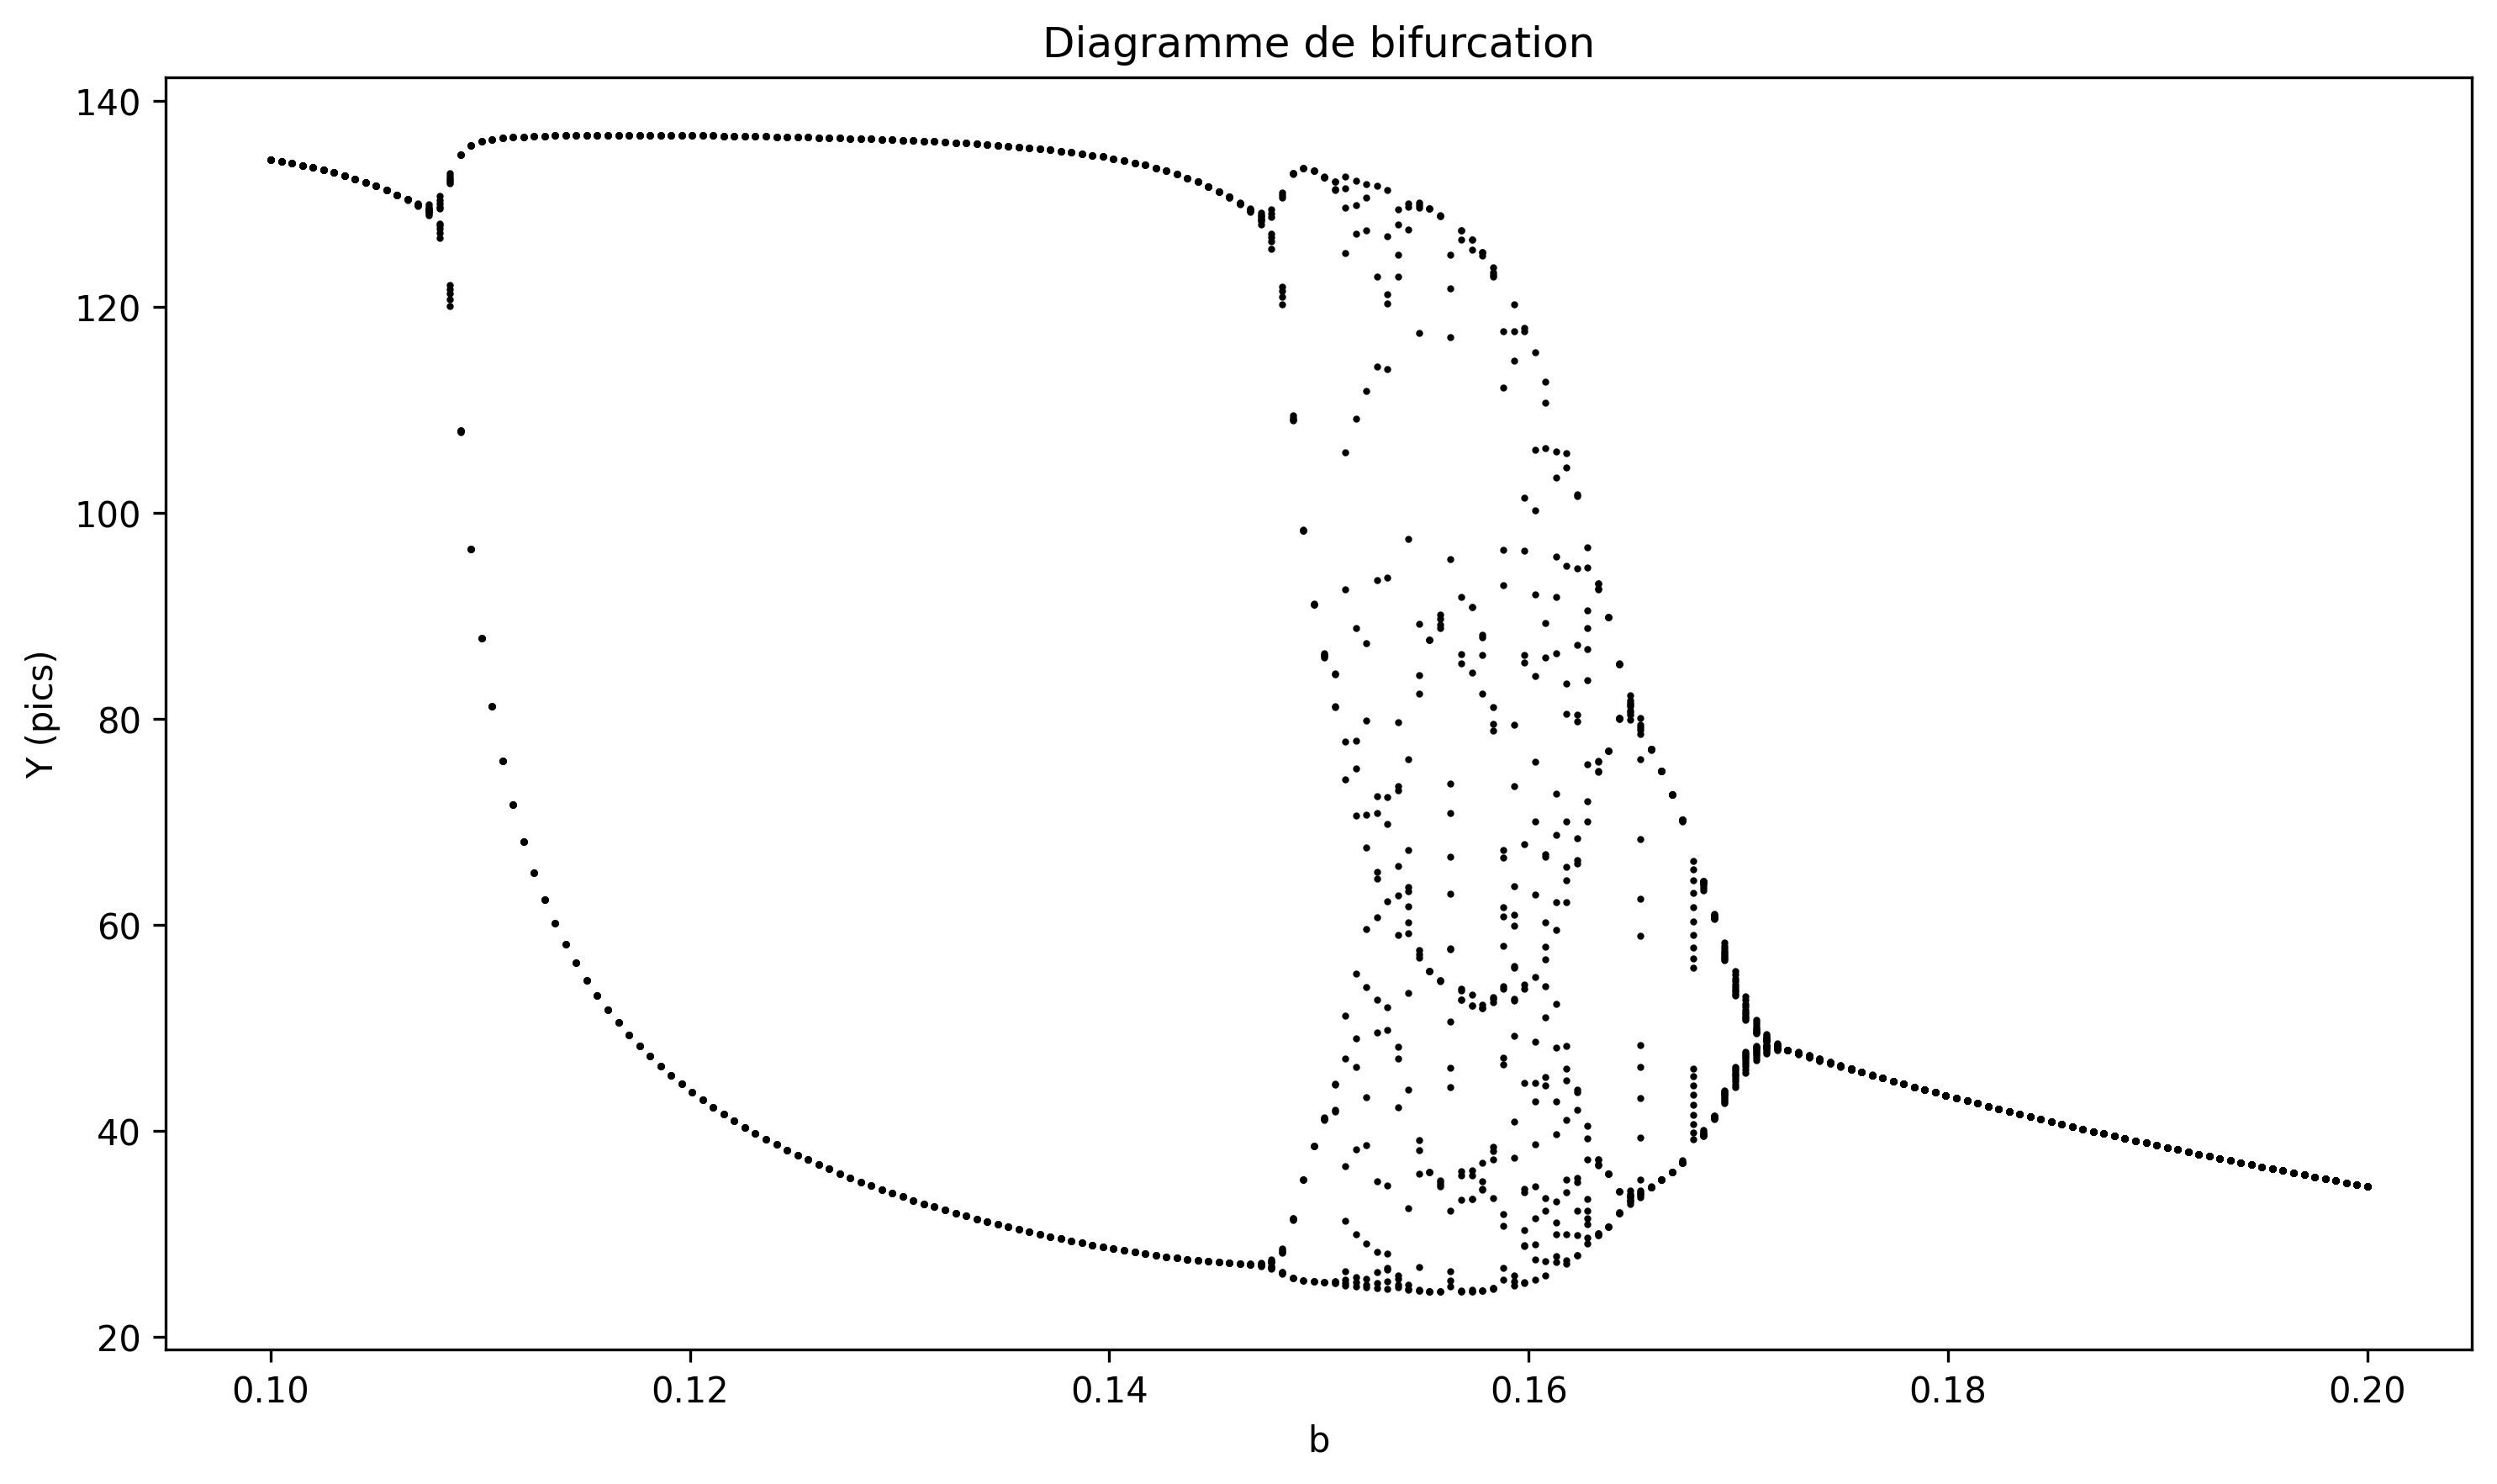
\includegraphics[width=0.85\textwidth]{../code/bifurcation.png}
\caption{Diagramme de bifurcation en fonction de $b$}
\label{fig:bifurcation}
\end{figure}

On y voit clairement la transition d'un comportement périodique à un régime chaotique, avec une multiplication des attracteurs.

\subsection{Chaoticité et lien avec la période 3}

Selon le théorème de Li et Yorke (\textit{Period three implies chaos} \citep{reaction}), l'existence d'une période 3 implique du chaos. Ce n'est pas observé ici, mais les irrégularités et la sensibilité au paramètre $b$ suggèrent fortement une dynamique chaotique.

\subsection{Difficultés numériques}

La simulation de systèmes chaotiques pose plusieurs défis :
\begin{itemize}
    \item Sensibilité aux conditions initiales
    \item Propagation exponentielle des erreurs
    \item Choix critique du pas de temps
    \item Distinction entre chaos réel et bruit numérique
\end{itemize}
    
Nous avons utilisé un pas de $h = 10^{-6}$ avec RK4 pour limiter ces effets, mais les imprécisions restent inévitables dans les zones sensibles.